\documentclass[12pt]{article}
% Full article preamble (duplicated, no common file)
\usepackage{fontspec}
\usepackage[a4paper,margin=2.5cm,includefoot]{geometry}
\usepackage{polyglossia}
\usepackage{amsmath}
\usepackage{amssymb}
\usepackage{xcolor}
\usepackage{fancyhdr}
\usepackage{graphicx}
\usepackage{listings}
\usepackage[most]{tcolorbox}
\usepackage{pifont}
\usepackage{enumitem}
\usepackage{titlesec}
\usepackage[bottom]{footmisc}
\usepackage{titling}
\usepackage{minted}
\usepackage{etoolbox}
\usepackage{array}
\usepackage{extsizes}

\newfontfamily\emoji{Segoe UI Emoji}

\pagestyle{fancy}

\setmainlanguage[numerals=western]{arabic}
\setotherlanguage{english}
\newfontfamily\arabicfont[Script=Arabic]{Amiri}
\newfontfamily\arabicfonttt[Script=Arabic]{Courier New}

\lstset{
  language=[Sharp]C,
  numbers=left,
  stepnumber=1,
  numbersep=8pt,
  frame=single,
  basicstyle=\ttfamily\small,
  keywordstyle=\color{blue},
  stringstyle=\color{red},
  commentstyle=\color{green!50!black}
}

\newif\ifdetailed
\ifdefined\setdetailed
  \setdetailed
\fi

\newif\ifwithsols
\ifdefined\setwithsols
  \setwithsols
\fi

% unified tcolorboxes for articles
\tcbset{colback=white, colframe=black, fonttitle=\bfseries, boxrule=0.8pt}
\newtcolorbox{boxDef}[1][]{colback=blue!5!white,colframe=blue!75!black,
  title={{\emoji📘} تعريف\ifx\\#1\\\else ~#1\fi :}}
\newtcolorbox{boxExercise}[1][]{colback=cyan!5!white,colframe=cyan!70!black,
  title={{\emoji🧩} تمرين\ifx\\#1\\\else ~#1\fi :}}
\newtcolorbox{boxExample}[1][]{colback=yellow!5!white,colframe=orange!90!black,
  title={{\emoji📝} مثال\ifx\\#1\\\else ~#1\fi :}}
\newtcolorbox{boxNote}[1][]{colback=gray!10!white,colframe=black,
  title={{\emoji✨} ملاحظة\ifx\\#1\\\else ~#1\fi :}}
\newtcolorbox{boxAttention}[1][]{colback=magenta!10!white,colframe=magenta!80!black,
  title={{\emoji🔔} تنبيه\ifx\\#1\\\else ~#1\fi :}}
\newtcolorbox{boxWarning}[1][]{colback=red!5!white,colframe=red!75!black,
  title={{\emoji⚡} ملاحظة هامة\ifx\\#1\\\else ~#1\fi :}}
\newtcolorbox{boxSolution}[1][]{colback=green!5!white,colframe=green!60!black,
  title={{\emoji✅} حل\ifx\\#1\\\else ~#1\fi :}}
\newtcolorbox{boxSymbol}[1][]{colback=purple!5!white,colframe=purple!70!black,
  title={{\emoji🔣} رمز\ifx\\#1\\\else ~#1\fi :}}

\tcbset{simplecode/.style={ colback=gray!5, colframe=black!50, boxrule=0.4pt, arc=2pt, left=4pt,right=4pt,top=4pt,bottom=4pt}}
\newenvironment{boxCode}{\begin{tcolorbox}[simplecode]}{\end{tcolorbox}}

\newcolumntype{C}[1]{>{\centering\arraybackslash}p{#1}}

% redefine spaces after titles
\makeatletter
\renewcommand{\@maketitle}{%
  \begin{center}
    {\huge \bfseries \@title \par}%
    \vskip 0.2em % space between title and author
    {\large \@author \par}%
    % \vskip 0.2em % space between author and date
    % {\normalsize \@date \par}%
  \end{center}
}
\makeatother

\fancyhf{} % clear default
\fancypagestyle{plain}{
  \fancyhf{}
  \fancyhead[L]{مدرسة التسامح الشاملة}
  % \fancyhead[L]{
\includegraphics[height=1cm]{../../../images/logoTasamoh.png}}
  \fancyhead[R]{الأستاذ محمود اغبارية}
  \fancyfoot[C]{\thepage}
}

\fancyhead[L]{مدرسة التسامح الشاملة}
\fancyhead[R]{الأستاذ محمود اغبارية}
\fancyfoot[C]{\thepage}
% \date{\today}

\setcounter{tocdepth}{3} % only section subsection and subsubsection in TOC


% ----------------------


% \begin{document}

% \maketitle

% % \clearpage  % start TOC on a new page
% % \renewcommand{\contentsname}{جدول المحتويات}
% % \tableofcontents
% % \clearpage

% \part*{part 1} % the * prevents numbering
% \section*{مقدمة}
% \subsection*{مثال رياضي}
% \subsubsection*{مثال فرعي}
% \paragraph*{ paragraph 1}
% \subparagraph*{sub paragraph 1}

% \ifdetailed
% \begin{english}
% \begin{minted}{csharp}
% // C# Example
% \end{minted}
% \end{english}
% \fi

% OLD WAY
% \ifdetailed
% \begin{english}
% \begin{lstlisting}
% // C# Example
% \end{lstlisting}
% \end{english}
% \fi

% % 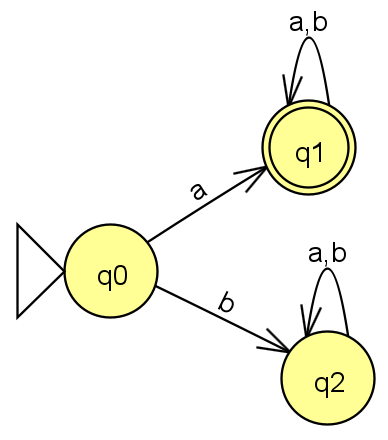
\includegraphics[width=0.2\textwidth]{../../../images/DFAs/ex1_q1.png}



% \vspace{3cm}
% \begin{flushleft}
% أرجو لكم وقتًا ممتعًا.

% الأستاذ محمود اغبارية.
% \end{flushleft}


% \end{document}



\title{موديلات حسابية}

\begin{document}

\maketitle

\renewcommand{\contentsname}{جدول المحتويات}
\tableofcontents
\clearpage

\section{مقدّمة}

\begin{itemize}
    \item موضوع النماذج الحسابية هو موضوع نظري، لا يوجد فيه برمجة.
    \item هدف الموضوع هو وصف الحاسوب بطريقة رياضية حتى نستطيع فحص حدود إمكانياته.
    \item هل يستطيع الحاسوب حل أي مشكلة حسابية؟ (الجواب لا طبعا)
    \item قبل أن نصل إلى نموذج الحاسوب (ماكنة تيورنج) نتعرف على نماذج أضعف من الحاسوب (قدرتها الحسابية أقل من قدرة الحاسوب)
    \item الموديل هو تخطيط يصف طريقة عمل شيء معين.
    \item مهمة حسابية هي مهمة هدفها معالجة المدخلات حتى تعطي نتيجة بناء على هذه المدخلات.
    \item في موضوع نماذج حسابية، نهتم بالمشاكل الحسابية التي تكون نتيجتها ثنائية (نعم أو لا - مقبول أو مرفوض\ldots)
\end{itemize}

\clearpage
\part{أوتومات نهائي}
\section{أوتومات نهائي محدّد (DFA)}

\subsection{أمثلة لموديلات تصف أشياء في حياتنا}

\paragraph{مثال 1:} كبسة المصباح لها حالتان، ننتقل من حالة إلى حالة عن طريق الضغط على الزر
\begin{center}
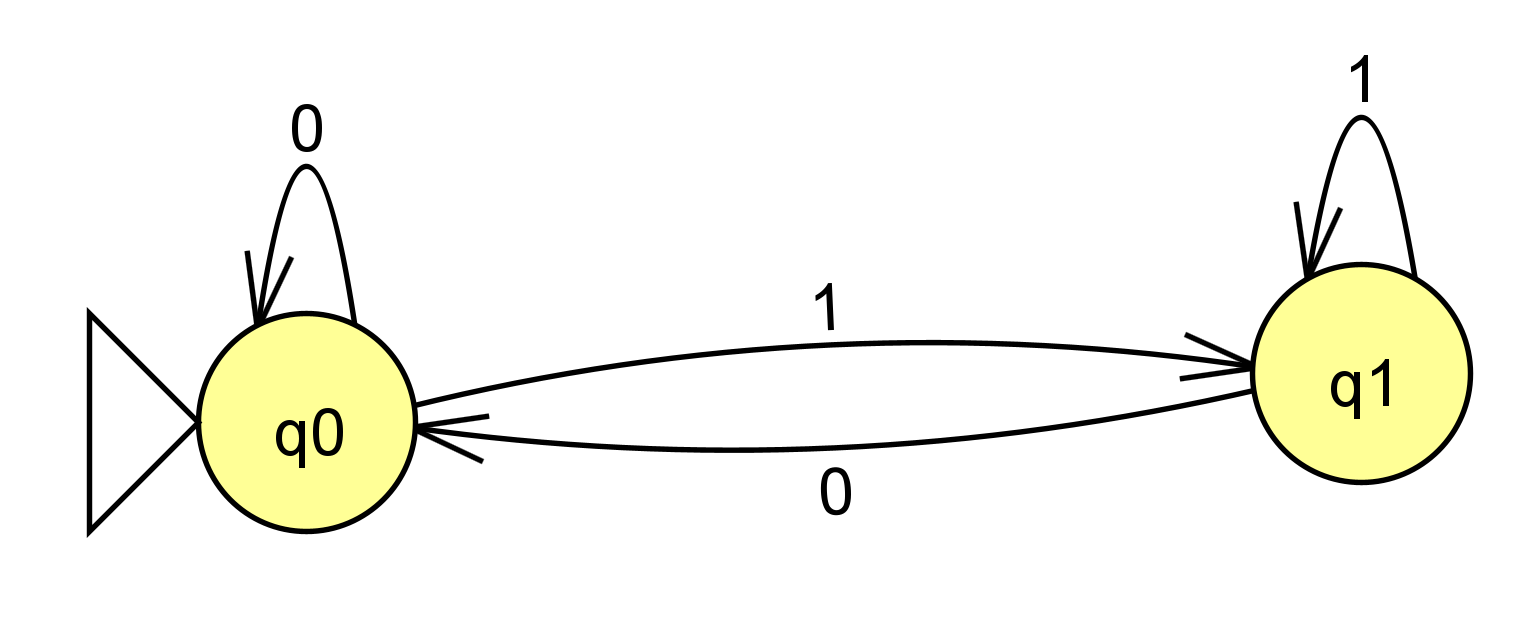
\includegraphics[width=0.3\textwidth]{../../../images/DFAs/01_lamp_dfa.png}
\end{center}

\paragraph{مثال 2:} موقف سيارات له بوابتان، يمكن الدخول فقط إذا كانتا مفتوحتين في نفس الوقت
\begin{center}
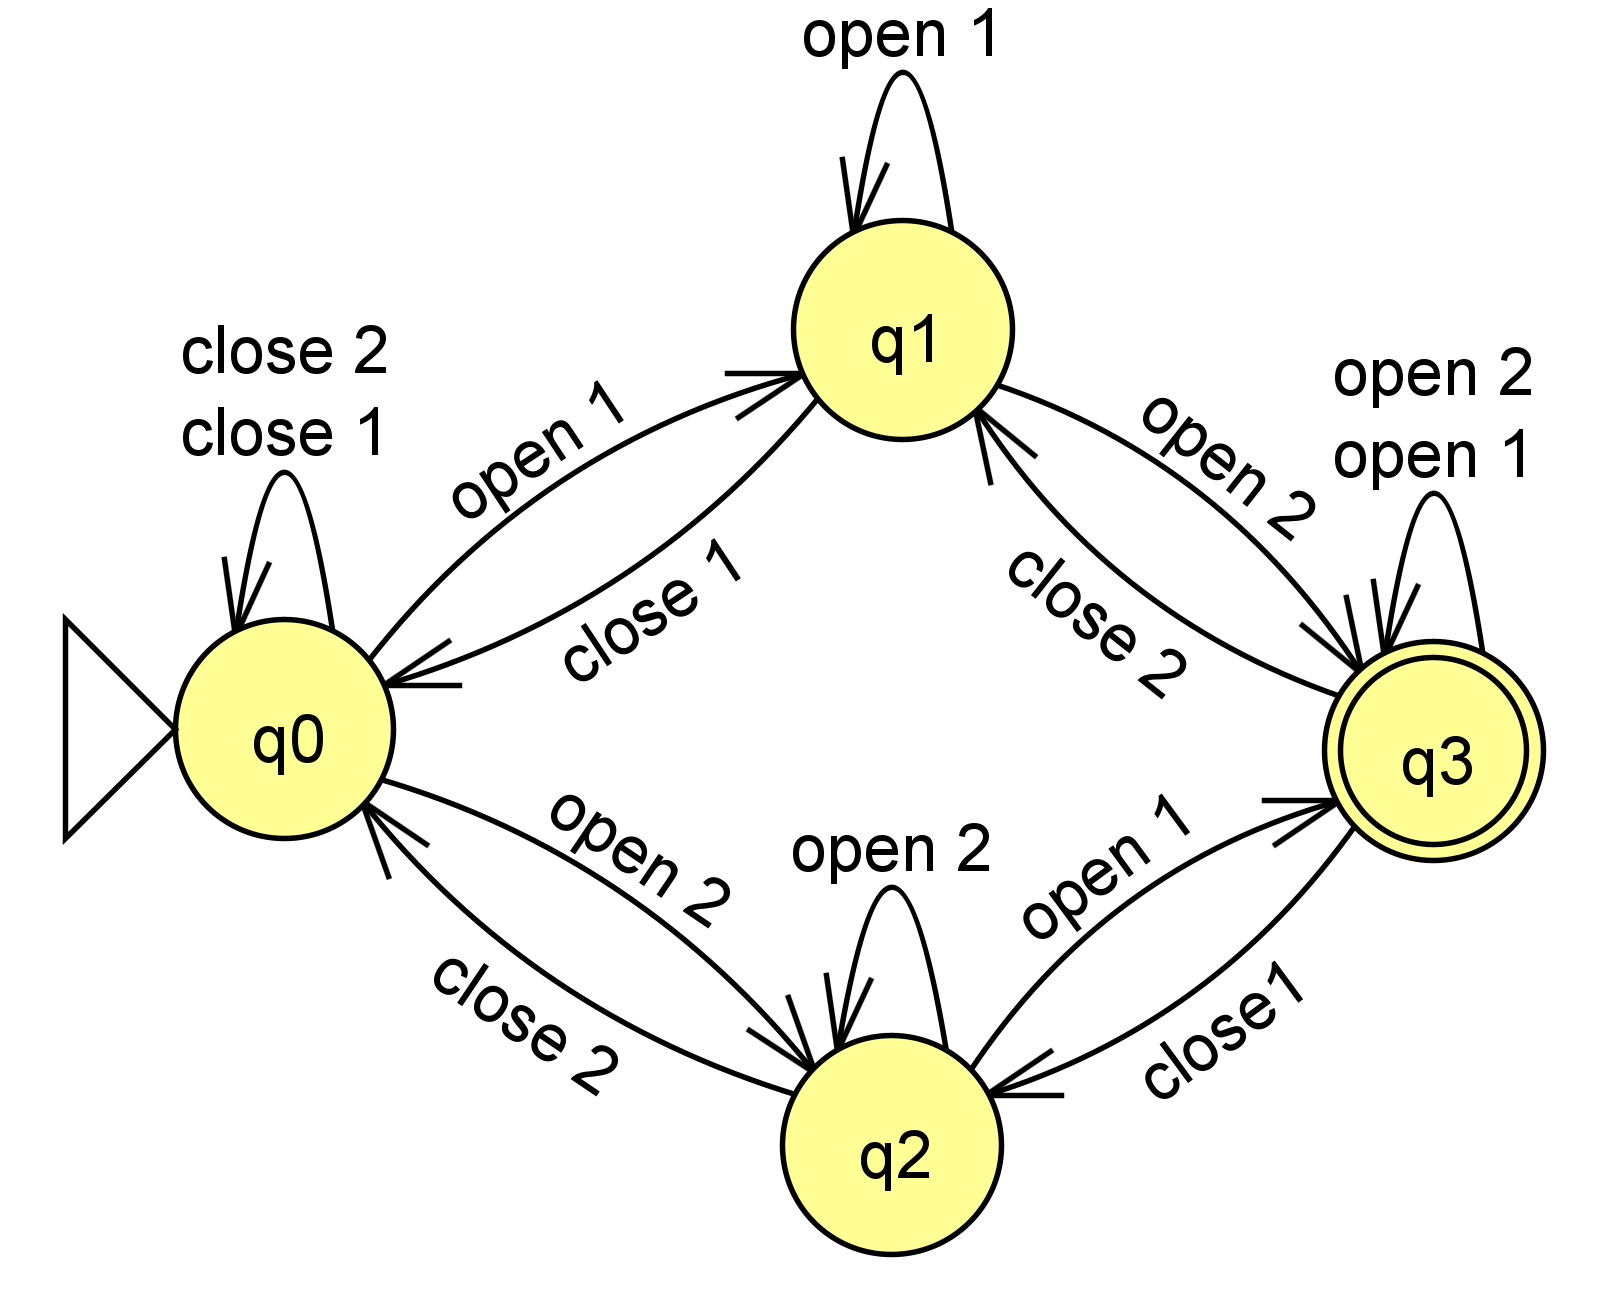
\includegraphics[width=0.5\textwidth]{../../../images/DFAs/02_two_gates_to_open_dfa.png}
\end{center}

\begin{itemize}
    \item $\mathtt{open 1}$ يعني فتح البوابة الأولى
    \item $\mathtt{close 1}$ يعني إغلاق البوابة الأولى
    \item $\mathtt{open 2}$ يعني فتح البوابة الثانية
    \item $\mathtt{close 2}$ يعني إغلاق البوابة الثانية
\end{itemize}

كل حالة في الأوتومات تمثل حالة معينة للبوابتين، أي لها معنى محدّد:
\begin{itemize}
    \item $q0$ يمثل الحالة التي فيها كلا البوابتين مغلقتان
    \item $q1$ يمثل الحالة التي فيها البوابة 1 مفتوحة، والبوابة 2 مغلقة
    \item $q1$ يمثل الحالة التي فيها البوابة 1 مغلقة، والبوابة 2 مفتوحة
    \item $q3$ يمثل الحالة التي فيها كلا البوابتين مفتوحتان
\end{itemize}


\paragraph{مثال 3:} هناك حاجز مكون من خشبات واقفة بشكل عمودي بجانب بعضها، كل خشبة مدهونة بلون واحد من الألوان أخضر، أحمر، أزرق. نريد بناء أوتومات يستقبل ألوان الخشبات للحاجز، ويقرر هل حالة دهن هذا الحاجز مقبول أم لا؟
نعتبر الحاجز مقبولا فقط إذا لم تكن هناك خشبتان متجاورتان لهما نفس اللون.

نبني موديلا يقرأ ألوان الخشبات بالترتيب. ونرمز للألوان بالأحرف: R للأحمر، G للأخضر، B للأزرق.

\begin{center}
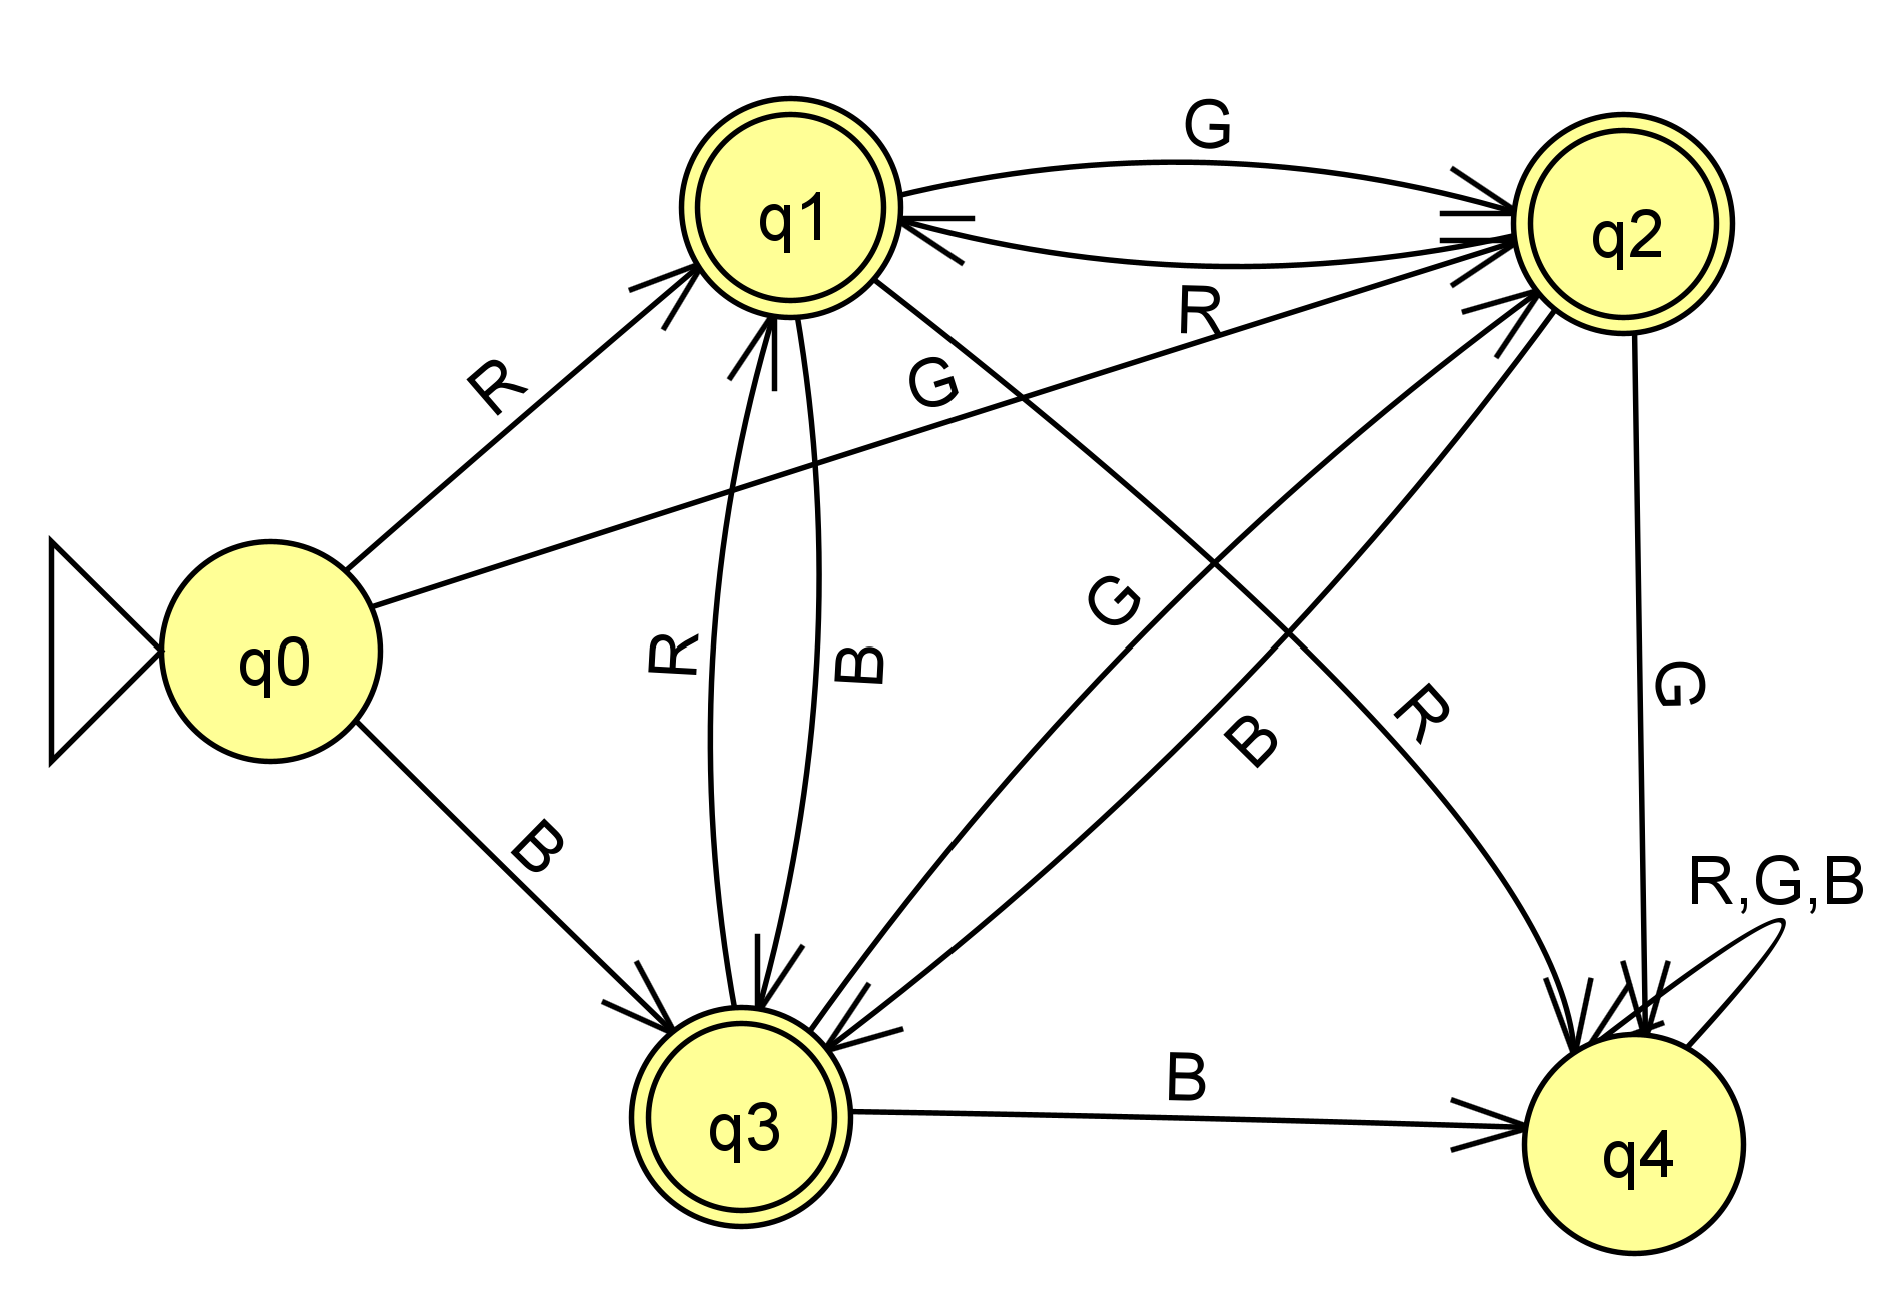
\includegraphics[width=0.5\textwidth]{../../../images/DFAs/03_color_series_dfa.png}
\end{center}

\begin{itemize}
    \item الذي يهمنا في هذه الحالة هو: ما هو آخر لون رأيناه؟ الألوان التي قبل ذلك لا تهمّنا.
    \item كل واحد من الحالات $q_1, q_2, q_3$ يمثل اللون الأخير الذي رأيناه:
    \begin{itemize}
        \item $q1$ يشير إلى أنّ اللون الأخير الذي رأيناه هو الأحمر
        \item $q2$ يشير إلى أنّ اللون الأخير الذي رأيناه هو الأخضر
        \item $q3$ يشير إلى أنّ اللون الأخير الذي رأيناه هو الأزرق
    \end{itemize}
    \item في كل واحد من هذه الحالات الثلاثة: إذا رأينا اللون الذي تمثله هذه الحالة مرة أخرى، فإنّنا نكون رأينا نفس اللون مرتين متتاليتين، وبالتالي فإنّ هذا المُدخَل غير قانوني (يوجد فيه خشبتان متجاورتان لهما نفس اللون).
    في هذه الحالة ننتقل إلى $q_4$ الذي يمثل حالة الفخّ، أي أنّنا لن نخرج منها أبدًا، وسنحكم على المدخل بأنّه غير قانوني.
    \item بالمقابل، إذا لم نصل إلى الحالة $q_4$ فإنّ هذا يعني أنّ المدخل كان قانونيًا ومقبولًا - لذلك نجعل الحالات الثلاثة $q_1, q_2, q_3$ كلها حالات قبول (ويظهر هذا في الرسم بجعلها دوائر مزدوجة.)
\end{itemize}


\subsection{الوصف الرياضي للأوتومات}

نعرّف مثلًا الأوتومات في المثال 3:

يمكننا وصف الأوتومات بأنّه مكون من المجموعات التالية:

\begin{enumerate}
    \item مجموعة الحالات:
    $$Q = \{q0, q1, q2, q3, q4\}$$

    \item الحالة الابتدائية:
    $$Start = q0$$

    \item مجموعة الحروف التي يتكون منها المدخل:
    $$ \Sigma = \{R,G,B\}$$

    \item الحالات القابلة
    $$ F = \{q1, q2, q3\}$$

    \item دالة الانتقالات بين الحالات:
    $$\delta: \{Q \times \Sigma \} \to Q$$
    هذه الدالة تستقبل: الحالة الحالية مع الحرف التالي في المدخل، وتخبرنا إلى أي حالة علينا الانتقال. \\
    يمكن وصف هذه الدالة عن طريق الجدول التالي:
    \begin{table}[h]
    \centering
    \begin{tabular}{|c|c|c|c|}
    \hline
    \textbf{الحالة} & \textbf{R} & \textbf{G} & \textbf{B} \\
    \hline
    $q0$ & $q1$ & $q2$ & $q3$ \\
    \hline
    $q1$ & $q4$ & $q2$ & $q3$ \\
    \hline
    $q2$ & $q1$ & $q4$ & $q3$ \\
    \hline
    $q3$ & $q1$ & $q2$ & $q4$ \\
    \hline
    $q4$ & $q4$ & $q4$ & $q4$ \\
    \hline
    \end{tabular}
    \end{table}
\end{enumerate}

\subsection{لغة الأوتومات}

عندما نشغّل الأوتومات على مُدخَل معيّن، فإنّنا نقول إن الأوتومات \textbf{قبل المدخل} أو \textbf{قبل الكلمة} إذا كان الأوتومات موجودًا في حالة قابلة عند الانتهاء من قراءة الكلمة (المدخل).

\paragraph{لغة الأوتومات: } هي مجموعة كل الكلمات التي يقبلها الأوتومات.

مثلًا، في المثال 3 أعلاه: لغة الأوتومات هي مجموعة كل الكلمات المكونة من الحروف R,G,B بحيث لا يوجد حرفان متشابهان متجاوران.

عادة، نرمز للغة الأوتومات بالحرف $L$.

\section{اللغات}

\subsection{مقدمة في علم المجموعات \textenglish{\texttt{Set Theory}}}

المجموعة هي تجميع لعناصر  (عادة تجمعها علاقة، أي تكون من نفس العالَم) نريد التعامل معها كوحدة واحدة. على سبيل المثال:
\begin{itemize}
    \item مجموعة الأعداد الزوجية: {0, 2, 4, 6, \ldots}
    \item مجموعة الأحرف العربية: {أ، ب، ت، ... ي}
    \item مجموعة الأرقام الصحيحة: {0، 1، 1-، 2، 2-، \ldots}
\end{itemize}

مثلًا، نعرّف المجموعات التالية
$$S1 = \{ 1, 2, 3, 4, 5, 6 \}$$
$$S2 = \{ 2, 4, 6 \}$$
$$S3 = \{ 5, 6, 7 \}$$
$$S4 = \{ 5, 6, 7 \}$$

\subsubsection{تعريفات ورموز وعمليات في علم المجموعات}

\begin{itemize}
\item المجموعة الخالية هي المجموعة التي لا تحتوي على أي عنصر، نرمز لها عادة بالحرف اليوناني $\emptyset = \{\}$ (في).

\item $a \in A$: العنصر ينتمي للمجموعة\\
أي أنّ العنصر $a$ موجود في المجموعة $A$. \\
مثلًا، في المجموعات أعلاه: $3 \in S1$

\item $a \notin A$: العنصر \textbf{لا} ينتمي للمجموعة \\
أي أنّ العنصر $a$ \textbf{غير موجود} في المجموعة $A$. \\
مثلًا، في المجموعات أعلاه: $7 \notin S1$

\item $A \subseteq B$: مجموعة تحتوي مجموعة أخرى (أو: مجموعة هي مجموعة جزئية لمجموعة أخرى) \\
أي أن المجموعة $B$ تحتوي المجموعة $A$. بكلمات أخرى: كل عنصر موجود في المجموعة $A$ فهو بالضرورة موجود أيضًا في المجموعة $B$.\\
مثلًا، في المجموعات أعلاه: $S2 \subseteq S1$

\item $A \nsubseteq B$: مجموعة \textbf{لا} تحتوي مجموعة أخرى (أو: مجموعة هي ليست مجموعة جزئية لمجموعة أخرى) \\
أي أنّ هناك عناصر موجودة في $A$ لكنها غير موجودة في $B$. \\
مثلًا، في المجموعات أعلاه: $S3 \nsubseteq S1$

\item $A = B$: مساواة بين مجموعتين \\
أي أنّ كل العناصر الموجودة في $A$ موجودة في $B$، والعكس أيضًا: كل عنصر في $B$ موجود في $A$ أيضًا. \\
مثلًا، في المجموعات أعلاه: $S3 = S4$

\item $|A|$: حجم المجموعة \\
أي عدد العناصر المختلفة في هذه المجموعة. \\
مثلًا، في المجموعات أعلاه: $|S1| = 6$ و $|S2| = |S3| = |S4| = 3$.

\item $A \cup B$: اتحاد مجموعتين \\
أي المجموعة المكونة من كل العناصر الموجودة في $A$ مع كل العناصر الموجودة في $B$. \\
مثلًا، في المجموعات أعلاه: $S2 \cup S3 = \{2, 4, 5, 6, 7 \}$.

\item $A \cap B$: تقاطع مجموعتين \\
أي المجموعة المكونة من كل العناصر الموجودة في المجموعة $A$ وفي المجموعة $B$ في نفس الوقت. \\
مثلًا، في المجموعات أعلاه: $S2 \cap S3 = \{6 \}$. لأنّه فقط العنصر 6 موجود في كلا المجموعتين.

\item $A \setminus B$: الفرق بين مجموعتين \\
أي المجموعة المكونة من كل العناصر الموجودة في المجموعة $A$ وليست موجودة في المجموعة $B$. \\
مثلًا، في المجموعات أعلاه: $S2 \setminus  S3 = \{2, 4 \}$. لأنّه فقط العنصر 6 موجود في كلا المجموعتين.

\end{itemize}

\paragraph{ملاحظات:}
\begin{itemize}
    \item المجموعة الخالية هي مجموعة جزئية لكل مجموعة أخرى $\emptyset \subseteq A$ لكل مجموعة $A$.
    \item كل مجموعة هي مجموعة جزئية لنفسها $A \subseteq A$.
    \item في المجموعات لا توجد أهمية للترتيب
    \item في المجموعات كل عنصر يظهر مرة واحدة (لا يوجد تكرار)
\end{itemize}

\paragraph{كتابة تعريف للمجموعة:}
عادة نكتب تعريفًا للمجموعة على الشكل التالي:
$$A = \{ x | x \text{شرط على } \}$$

\textbf{مثال:}
في المجموعات التي عرفناها أعلاه، يمكننا أن نعرف:
$$S2 = \{ x \in S1 | x\%2=0 \}$$


\subsection{رموز وتعريفات في اللغات}

\subsubsection{الأبجدية}

\begin{boxDef}
    \paragraph{الأبجدية} هي مجموعة نهائية وغير فارغة من الرموز (الرموز يمكن أن تكون أي رموز: أرقام، أحرف، علامات ترقيم...).
\end{boxDef}
\begin{boxSymbol}
    عادة نرمز للأبجدية بالحرف $\Sigma$ (سيجما).
\end{boxSymbol}

مثلًا:
\begin{itemize}
    \item $\Sigma = \{a, b\}$ هي أبجدية مكونة من رمزين اثنين (حرفَين)
    \item $\Sigma = \{0, 1\}$ هي أبجدية مكونة من رمزين اثنين أيضًا (في هذه الحالة رقمين)
    \item $\Sigma = \{0, 1, 2, \dots, 9\}$ هي أبجدية مكونة من عشرة رموز (الأرقام).
\end{itemize}


\subsubsection{الكلمة}

\begin{boxDef}
    \paragraph{الكلمة} هي تسلسل من الرموز من أبجدية معينة.
\end{boxDef}

مثلًا، بالنسبة للأبجدية $\Sigma = \{0, 1\}$ فإن السلاسل التالية هي كلمات مكونة من هذه الأبجدية:
\begin{itemize}
    \item $w_1 = 000$
    \item $w_2 = 111000$
    \item $w_3 = 1010$
    \item $w_4 = 01011$
\end{itemize}

\begin{boxAttention}
    الكلمات أعلاه ليست أرقامًا، لا نقول إن الكلمة $w_1$ هي صفر، بل هي كلمة مكونة من ثلاثة رموز كلها صفر.
\end{boxAttention}

\begin{boxSymbol}
    نستحدم الرمز $|w|$ للتعبير عن عدد الرموز في الكلمة $w$.
\end{boxSymbol}
مثلًا، في الكلمات أعلاه:
\begin{itemize}
    \item $|w_1| = 3$
    \item $|w_2| = 6$
    \item $|w_3| = 4$
    \item $|w_4| = 5$
\end{itemize}

\begin{boxSymbol}
    الكلمة قد تكون فارغة، أي لا يوجد فيها أي رموز. \\
    نرمز للكلمة فارغة بالحرف $\epsilon$ (إبسيلون).
\end{boxSymbol}
حسب التعريف في النقطة السابقة: $|\epsilon| = 0$ لأنّ عدد الرموز في الكلمة الفارغة هو 0.

\begin{boxSymbol}
    نستعمل الرمز $\#_a(w)$ للتعبير عن عدد المرات التي يظهر فيها الحرف $a$ في الكلمة $w$.
\end{boxSymbol}
مثلًا، في الكلمات أعلاه:
\begin{itemize}
    \item $\#_1(w_0) = 0$ و $\#_0(w_0) = 3$
    \item $\#_1(w_1) = 3$ و $\#_0(w_1) = 4$
    \item $\#_1(w_2) = 2$ و $\#_0(w_2) = 2$
    \item $\#_1(w_3) = 3$ و $\#_0(w_3) = 2$
\end{itemize}

\begin{boxSymbol}
    نستعمل الرمز $R(w)$ أو $w^R$ للتعبير عن الكلمة المعكوسة من $w$. (أي نقرأ $w$ من اليمين إلى اليسار)
\end{boxSymbol}
مثلًا، في الكلمات أعلاه:
\begin{itemize}
    \item $R(w^1) = w^R_1 = 000$
    \item $R(w^2) = w^R_2 = 000111$
    \item $R(w^3) = w^R_3 = 0101$
    \item $R(w^4) = w^R_4 = 11010$
\end{itemize}

\subsubsection{اللغة}

\paragraph{اللغة} هي مجموعة من الكلمات المعرفة فوق أبجدية معيّنة.

مثلًا:
$L_1 = \{0, 1, 01, 10\}$ معرفة فوق الأبجدية $\Sigma = \{0, 1\}$.

اللغة يمكن أن تكون:
\begin{itemize}
    \item لغة \textbf{منتهية} (عدد كلماتها محدود).
    \item لغة \textbf{غير منتهية} (عدد كلماتها غير محدود).
\end{itemize}

\subsection{عمليات على الأبجدية واللغات والكلمات}

\begin{enumerate}

\item
    \textbf{عملية القوة على الأبجدية} $\Sigma^n$: جميع الكلمات الممكنة من الأبجدية $\Sigma$ بطول $n$.

    مثال: إذا كانت $\Sigma = \{0,1\}$:
    \begin{itemize}
        \item $\Sigma^1 = \{0, 1\}$ كل الكلمات التي يمكن تكوينها بطول 1 من رموز الأبجدية $\Sigma$.
        \item $\Sigma^2 = \{00, 01, 10, 11\}$ كل الكلمات التي يمكن تكوينها بطول 2 من رموز الأبجدية $\Sigma$.
        \item $\Sigma^3 = \{000, 001, 010, 011, 100, 101, 110, 111\}$ كل الكلمات التي يمكن تكوينها بطول 3 من رموز الأبجدية $\Sigma$.
    \end{itemize}

\item
    \textbf{مجموعة كل الكلمات فوق الأبجدية} $\Sigma^*$: جميع الكلمات الممكنة من أي طول (بما في ذلك الكلمة الفارغة) فوق الأبجدية $\Sigma$.

    مثال: $\Sigma = \{a, b\}$
    $\Sigma^* = \{\epsilon, a, b, aa, ab, ba, bb, aaa, aab, \dots\}$

\item
    \textbf{ضرب / إلصاق الكلمات واللغات}
    \begin{itemize}
        \item \textbf{ضرب كلمتين:} هو ما ينتج عند إلصاق الكلمة الثانية بالأولى، أي نكتب كل رموز الكلمة الأولى ثم بعدها نكتب كل رموز الكلمة الثانية. \\
        مثلًا: إذا كان $u = 010$ و $v = 11$، فإن $uv = 01011$.
        \item \textbf{ضرب لغتين:} الناتج هو اللغة المكونة من الكلمات الناتجة عن إلصاق كل كلمة من اللغة الأولى مع كل كلمة من اللغة الثانية. \\
        مثلًا: إذا كان $L_1 = \{00,11\}$ و $L_2 = \{aa,bb\}$ فإن: $L_1L_2 = \{00aa, 00bb, 11aa, 11bb\}$
    \end{itemize}

\item
    \textbf{عملية القوة على اللغة:} $L^n$ هي عملية ضرب (إلصاق) اللغة بنفسها $n$ مرات. \\
    مثلًا: إذا كانت $L = \{a,b\}$:
    \begin{itemize}
        \item $L^1 = \{a,b\}$
        \item $L^2 = \{aa, ab, ba, bb\}$
        \item $L^3 = \{aaa, aab, aba, abb, baa, bab, bba, bbb\}$
    \end{itemize}

\item
    \textbf{عملية القوة على الحرف:} $a^n$ هي عملية ضرب (إلصاق) الحرف $a$ بنفسه $n$ مرات. \\
    مثلًا:
    \begin{itemize}
        \item $a^1 = a$
        \item $a^2 = aa$
        \item $a^3 = aaa$
        \item $a^0 = \epsilon$ (أي الكلمة الفارغة)
    \end{itemize}

\item
    \textbf{عملية النجمة على اللغة:} $L^*$ هي مجموعة كل الكلمات التي يمكن تكوينها من ضرب (إلصاق) أي عدد من الكلمات من اللغة $L$ مع بعضها البعض (بما في ذلك الكلمة الفارغة). \\
    مثلًا: إذا كانت $L = \{aa,bb\}$ فإن: \\
    $L^* = \{\epsilon, aa, bb, aaaa, aabb, bbaa, bbbb, aaaaaa, aaaabbbb, aabbaabb, \dots\}$

\item
    \textbf{عملية النجمة على الحرف:} $a^*$ هي مجموعة كل الكلمات التي يمكن تكوينها من ضرب (إلصاق) أي عدد من الحرف $a$ مع نفسه (بما في ذلك الكلمة الفارغة). \\
    مثلًا: $a^* = \{\epsilon, a, aa, aaa, aaaa, aaaaa, \dots\}$

\item \textbf{عملية زائد على الأبجدية / اللغة / الحرف:}
    لها نفس معنى النجمة إلّا أن التكرار يجب أن يكون مرة واحدة على الأقل.
    \textbf{أي أنّ النتيجة لا تشمل الكلمة الفارغة}.
    مثلًا:
    \begin{itemize}
        \item إذا كانت $\Sigma = \{a,b\}$ فإن: $\Sigma^+ = \{a, b, aa, ab, ba, bb, aaa, aab, \dots\}$.
        \item إذا كانت $L = \{aa,bb\}$ فإن:\\
        $L^+ = \{aa, bb, aaaa, aabb, bbaa, bbbb, aaaaaa, aaaabbbb, aabbaabb, \dots\}$.
        \item $a^+ = \{a, aa, aaa, aaaa, aaaaa, \dots\}$.
    \end{itemize}

\end{enumerate}

\subsubsection{أمثلة}

نفترض أنّ الأبجدية هي $\Sigma = \{a, b\}$ لكل اللغات التالية.

\begin{itemize}
    \item $L = \{a^m | m \geq 0 \}$ \\
    هي مجموعة كل الكلمات التي تتكون من الحرف $a$ فقط (أي لا يوجد فيها الحرف $b$) بأي طول (بما في ذلك الكلمة الفارغة). \\
    مثلًا:
    \begin{itemize}
        \item $\epsilon , a, aa, aaa, aaaa$ كلها كلمات موجودة في اللغة.
        \item $b, ab, ba, aab, aba, baa$ كلها كلمات غير موجودة في اللغة.
    \end{itemize}

    \item $L = \{a^m | m > 0 \}$ \\
    هي مجموعة كل الكلمات التي تتكون من الحرف $a$ فقط (أي لا يوجد فيها الحرف $b$) بحيث يكون طول الكلمة أكبر من 0 (أي لا تشمل الكلمة الفارغة). \\
    الأمثلة السابقة صحيحة هنا أيضًا، إلا الكلمة الفارغة فهي غير موجودة في اللغة.

    \item $L = \{a^m b^n | m,n \geq 0 \}$ \\
    هي مجموعة الكلمات التي تتكون من صفر أو أكثر من الحرف $a$ متبوعة بصفر أو أكثر من الحرف $b$. \\
    لاحظ أنّ $m$ و $n$ يمكن أن يكونا صفرًا، وبالتالي فإنّ $a^0 b^0 = \epsilon$ (الكلمة الفارغة) موجودة في اللغة. \\
    مثلًا:
    \begin{itemize}
        \item $\epsilon$ موجودة في اللغة.
        \item $a, b, ab, aab, abb, aaabbb$ كلها كلمات موجودة في اللغة.
        \item $ba, aba, baa, bab, aaba$ كلها كلمات غير موجودة في اللغة.
    \end{itemize}
    \begin{boxNote}
    يمكن التعبير عن اللغة السابقة أيضًا بالشكل التالي:
    $L = \{a^* b^* \}$
    \end{boxNote}

    \item $L = \{a^m b^n | m,n > 0 \}$ \\
    هي مجموعة كل الكلمات التي تبدأ بالحرف $a$ بحيث يظهر مرة أو أكثر، ثم بعد ذلك يظهر الحرف $b$ مرة أو أكثر، ولا يظهر الحرف $a$ بعد ظهور الحرف $b$. \\
    مثلًا:
    \begin{itemize}
        \item $\epsilon$ غير موجودة في اللغة.
        \item $ab, aab, abb, aaabbb$ كلها كلمات موجودة في اللغة.
        \item $a, b, aa, bb, ba, aba, baa, bab, aaba$ كلها كلمات غير موجودة في اللغة.
    \end{itemize}
    \begin{boxNote}
    يمكن التعبير عن اللغة السابقة أيضًا بالشكل التالي:
    $L = \{a^+ b^+ \}$
    \end{boxNote}

    \item $L = \{w \in \Sigma^* | w \text{ يحتوي على عدد زوجي من } a's \}$ \\
    هي مجموعة كل الكلمات التي تحتوي على عدد زوجي من الحرف $a$ (بما في ذلك 0). \\
    مثلًا:
    \begin{itemize}
        \item $\epsilon, b, bb, abba, aabb, baba, baabaabbb, ababaab$ كلها كلمات موجودة في اللغة.
        \item $a, aaab, abb, bab, aaba$ كلها كلمات غير موجودة في اللغة.
    \end{itemize}

    \item $L = \{w \in \Sigma^* | \left| w \right| \% 2 = 0 \}$ \\
    هي مجموعة كل الكلمات التي يكون طولها (عدد رموزها) زوجيًا (بما في ذلك 0). \\
    مثلًا:
    \begin{itemize}
        \item $\epsilon, ab, aa, bb, aabb, baba, baabaabb$ كلها كلمات موجودة في اللغة.
        \item $a, b, aaa, abb, bab, aabba$ كلها كلمات غير موجودة في اللغة.
    \end{itemize}

\end{itemize}

\begin{boxAttention}
    \begin{itemize}
        \item $\{\epsilon\}$ هي مجموعة مكونة من عنصر واحد فقط، هو الكلمة الخالية.
        \item $|\{\epsilon\}| = 1$ لأنّ عدد العناصر في المجموعة التي تحتوي على الكلمة الفارغة هو 1 (الكلمة الفارغة).
        \item $|\emptyset| = 0$ لأنّ عدد العناصر في المجموعة الخالية هو 0.
        \item $\epsilon \notin \emptyset$ لأنّ المجموعة الخالية لا تحتوي على أي عنصر.
        \item $\{\epsilon\} \neq \emptyset$.
    \end{itemize}
\end{boxAttention}

\end{document}
